\documentclass{article}

% Package Imports
\usepackage{amsmath}
\usepackage{graphicx}

% Config
\graphicspath{{./img/}}

% Preamble: Title Details
\title{Latex Tutorial}
\date{2023-10-25}
\author{Amanpreet Singh}

\begin{document}
  \pagenumbering{arabic}
  \maketitle %Insert Title
  \newpage %Break Page

\section{Introduction}
This is the introduction section.

\subsection{Subsection}
This is a subsection.  

\subsubsection{Sub Subsection}
This is a sub-subsection.

\paragraph{Paragraph} 
This is a Paragraph.

\subparagraph{Sub Para}
This is a Sub Paragraph

\section{Features}

\subsection{Packages}

\paragraph{Equations}
Equations Package Example.
\begin{equation}
  f(x) = x^2
\end{equation}

\paragraph{Embedding}
...
This formula $f(x) = x^2$ is an embedding.
...

\paragraph*{Double Line}

\begin{equation*}
  1 + 2 = 3 
\end{equation*}
\begin{equation*}
  1 = 3 - 2
\end{equation*}

\begin{align*}
  1 + 2 &= 3\\
  1 &= 3 - 2
\end{align*}

\subsection{Math}

\paragraph{Fractions}
\begin{align*}
  f(x) &= x^2\\
  g(x) &= \frac{1}{x}\\
  F(x) &= \int^a_b \frac{1}{3}x^3
\end{align*}

\subsection{Images}

\paragraph{Single}

\begin{figure}
  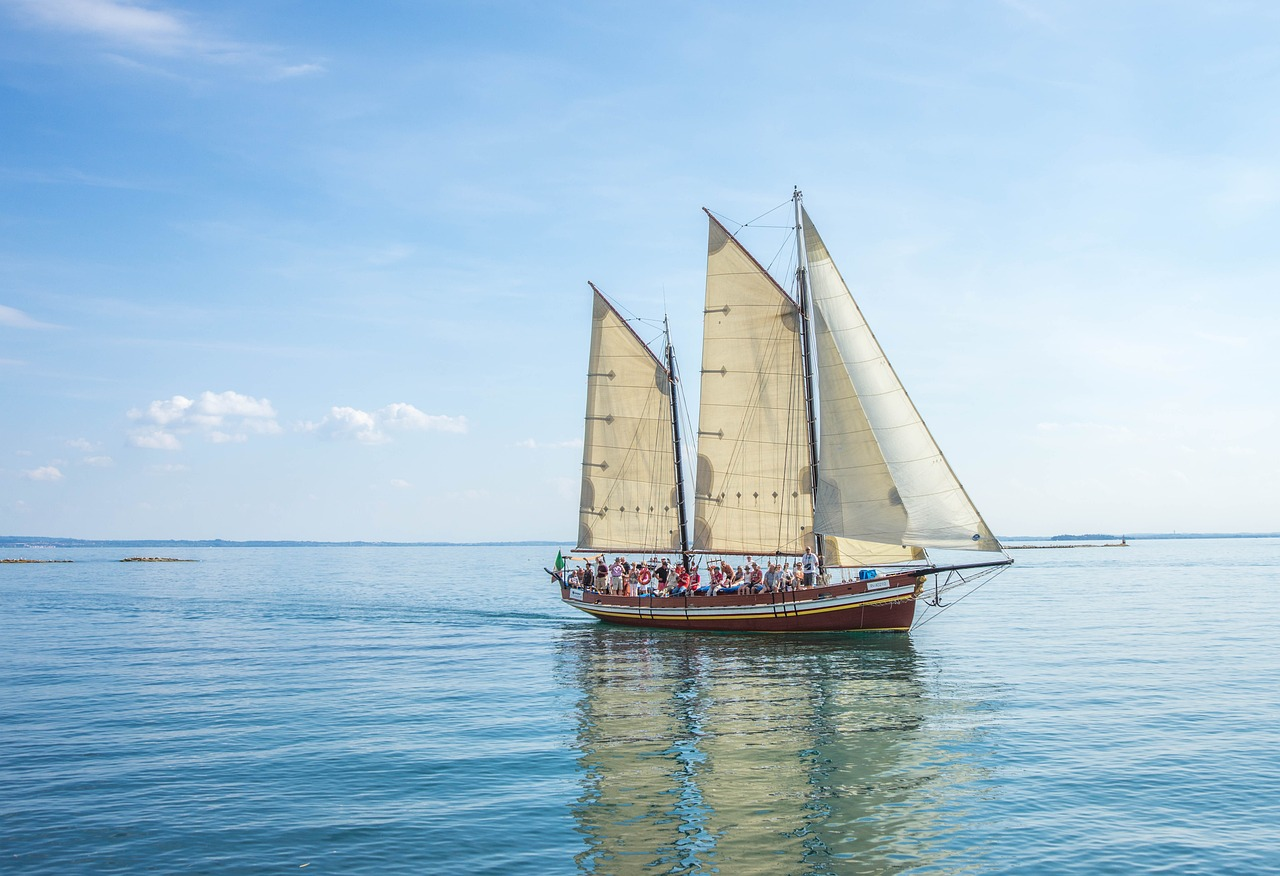
\includegraphics[width=\linewidth]{boat.jpg}
  \caption{Sail Boat.}
  \label{fig:boat1}
\end{figure}

Figure \ref{fig:boat1} shows a boat.


\end{document}